\documentclass[aspectratio=169]{beamer}

\usepackage{bashful}
\usepackage{fontspec}
\usepackage{listings}
\usepackage{tikz}

\usetikzlibrary{calc}
\usetikzlibrary{positioning}

\definecolor{solarizedRed}{RGB}{220, 50, 47}
\definecolor{solarizedYellow}{RGB}{181, 137, 0}
\definecolor{solarizedBlue}{RGB}{38, 139, 210}
\definecolor{solarizedGreen}{RGB}{133, 153, 0}
\definecolor{solarizedPurple}{RGB}{108, 113, 196}

\setbeamercolor{title}{fg=solarizedBlue}
\setbeamercolor{frametitle}{fg=solarizedBlue}
\setbeamercolor{structure}{fg=solarizedBlue}

\setbeamertemplate{navigation symbols}{}
\setbeamertemplate{headline}{}
\setbeamertemplate{footline}{}
\setbeamertemplate{itemize items}[circle]

\setbeamertemplate{footline}{
  \begin{tikzpicture}[remember picture,
                      overlay,
                      shift={(current page.south west)}]
    \node [black!50, inner sep=2mm, anchor=south east]
          at (current page.south east) {\large \insertframenumber};
  \end{tikzpicture}
}

\setsansfont{Overpass}[Scale=MatchLowercase]
\setmonofont{Overpass Mono}[Scale=MatchLowercase]

\lstset{
  basicstyle=\ttfamily,
  language=C,
  escapeinside={(*@}{@*)},
  commentstyle={\color{black!35}},
}

\setbeamertemplate{title page}
{
  \begin{tikzpicture}[remember picture,
                      overlay,
                      shift={(current page.south west)}]
    \node (title) [inner sep=0, scale=2, align=left]
          at (\paperwidth / 2, \paperheight * 2 / 3)
          {\bfseries \usebeamerfont{title}\usebeamercolor[fg]{title}Projact Pactum\\
           \usebeamerfont{title}\usebeamercolor[fg]{title}\inserttitle};
    \node (author) [scale=1.5] at (\paperwidth / 2, \paperheight / 3)
          {\insertauthor};
    \node [anchor=south east, inner sep=2mm] at (\paperwidth, 0)
          {\color{solarizedYellow} \texttt{\splice{../../../version.sh}}};
    \node [below=of title.west, anchor=north west, align=left]
          {\color{solarizedYellow} \insertdate};
  \end{tikzpicture}
}


\title{Weekly Meeting}
\date{November 6, 2020}
\author{Jon Eyolfson \and John Thorpe}

\begin{document}

  \begin{frame}[plain]
    \titlepage
  \end{frame}

  \setcounter{framenumber}{0}

  \begin{frame}
    \frametitle{Instance Types}

    Lack of scalability difference on ResNet32 using \texttt{p2} instances (last week)
    \begin{itemize}
      \item K80 GPUs don't support NCCL optimizations
      \begin{itemize}
        \item CPU communication performs \emph{better} than NCCL on K80s
      \end{itemize}
      \item NCCL perf-debug tests show poor throughput
    \end{itemize}

    \vspace{3em}
    NCCL throughput increase significant on \texttt{p3} instance (V100 GPU)
    \begin{itemize}
      \item Differences need to be accounted for if system heterogeneous
    \end{itemize}

  \end{frame}

  \begin{frame}
    \frametitle{ResNet 50 Scalability}

    \begin{center}
      \includestandalone[scale=1.25]{../../figures/resnet50-synthetic-scalability}
    \end{center}

    Scalability of the ResNet50 model using \texttt{p3 instances (V100s)}

  \end{frame}

  \begin{frame}
    \frametitle{Spot Instance Availability Over 8 Days}

    \begin{center}
      \includestandalone[scale=1.25]{../../figures/aws-availability-2020-10-21-to-2020-10-28}
    \end{center}

    \texttt{p2.xlarge} instance type in zone \texttt{us-east-1d} from
    Oct. 21 to 28
  \end{frame}

  \begin{frame}
    \frametitle{Spot Instance Availability Insights}

    \begin{tabular}{rl}
      \textbf{Mean:}               & 2.2 h   \\
      \textbf{Standard deviation:} & 2.0 h   \\
      \textbf{Median:}             & 1.0 h   \\
      \textbf{Max:}                & 9.1 h   \\
      \textbf{Uptime:}             & 47.33\% \\
    \end{tabular}

    \vspace{3em}

    \texttt{p2.xlarge} instances in \texttt{us-east-1d} aren't available for long

    \vspace{1em}

    Our design needs to include restarting from no spot instances
  \end{frame}

  \begin{frame}
    \frametitle{Current Design}

    \begin{columns}
      \column{0.25\textwidth}
      \begin{flushright}
        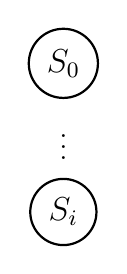
\begin{tikzpicture}[
          auto,
          node distance=1cm,
          server/.style={
            thick,
            circle,
            draw,
            font=\sffamily\large},
        ]
          \node[server] (1) {$S_0$};
          \node[server] (2) [below=of 1] {$S_i$};
          \path (1) -- node[auto=false] {\vdots} (2);
        \end{tikzpicture}
      \end{flushright}
      \column{0.75\textwidth}
      \begin{itemize}
        \item One global configuration
        \item Manual checkpointing
        \item Manual restarts
      \end{itemize}
    \end{columns}

    \vspace{3em}

    \hspace{7em} Note that Horovod will start computation on each server, $S$
  \end{frame}

  \begin{frame}
    \frametitle{Our Starter Design}

    \begin{columns}
      \column{0.5\textwidth}
      \begin{flushright}
        \begin{tikzpicture}[
          ->,
          >=stealth',
          shorten >=1pt,
          auto,
          node distance=1cm,
          server/.style={
            thick,
            circle,
            draw,
            font=\sffamily\large},
        ]
          \node[draw] (c) {Coordinator};
          \node[server] (1) [right=of c, yshift=2.5em] {$S_0$};
          \node[server] (2) [below=of 1] {$S_i$};
          \path (1) -- node[auto=false]{\vdots} (2);
          \path (c) edge (1);
          \path (c) edge (2);
        \end{tikzpicture}
      \end{flushright}
      \column{0.5\textwidth}
      \begin{itemize}
        \item Coordinator handles configuration
        \item Manual checkpointing
        \item Automatic restarts
      \end{itemize}
    \end{columns}

    \vspace{3em}

    \hspace{7em} Initially we'll be able to test a simple approach and evaluate
  \end{frame}

  \begin{frame}
    \frametitle{Scope}

    \begin{itemize}
      \item Small to Medium Models (fit on a single GPU)
      \item Data parallelism
      \item Homogeneous GPUs
      \item Synchronous operations
    \end{itemize}
  \end{frame}

  \begin{frame}
    \frametitle{Experiment Design}

    Test end-to-end time to a certain accuracy (approx. 12 hours)

    \begin{itemize}
      \item Test the best case scenario (no preemptions)
      \item Compare against manual preemptions with checkpointing

            (using our known AWS patterns)
    \end{itemize}

    \vspace{2em}

    The difference in end-to-end time should give us a good idea of feasibility
  \end{frame}

  \begin{frame}
    \frametitle{Future Directions}

    \begin{itemize}
      \item Large models (BERT large)
      \item Heterogeneous GPUs
      \item Model parallelism (splitting with preemption)
      \item Asynchronous operations
    \end{itemize}
  \end{frame}

\end{document}
